\documentclass[english,twoside, openright, hidelinks, 11 pt, class=report,crop=false]{standalone}
\input{../../preamb}



\begin{document}
{\Large Eksamen R2 Våren 2025\hfill  {\footnotesize Løsning fra \color{blue} \href{https://sindreheggen.wordpress.com/}{OpenMathBooks}}}	

\subsection*{Oppgave 1}
\abc{
\item 
\begin{align}
\int_{0}^{2} \left(e^{2x}+x\right)\deltax&=\left[\frac{1}{2}e^{2x}+\frac{1}{2}x^2\right]_0^2\br
&= \frac{1}{2}\left(e^{2\cdot2}+\cdot2^2\right)-\frac{1}{2}\left(e^0+0\right) \br
&=\frac{1}{2}(e^4+3)
\end{align}
\item Vi setter $u=\ln x$, da er $u'=\frac{1}{x}$. Dermed har vi at
\begin{align*}
	\int \frac{\sin(\ln x)}{x}\deltax &= \int \sin(u)u'\deltax \\
	&= \int \sin(u)\deltau \\
	&= -\cos(u) + C \\
	&= -\cos(\ln x) + C
\end{align*}
}

\subsection*{Oppgave 2}
\abc{
\item Vi har at
\[ f(x)= \int 2x^{-2}\deltax=-2x^{-1}+C \]
Videre er
\begin{align*}
	f(2)&=2 \\
	-2\cdot2^{-1} + C &= 2 \\
	C &= 3
\end{align*}
Dermed er
\[ f(x)=-2x^{-1}+3 \]
	\item Siden det er snakk om et areal avgrenset bare av grafene til to funksjoner, er det rimelig å anta at området er mellom to skjæringspunkt for grafene. Når $g(x)=h(x)$, er 
	\begin{align*}
		x &= -\frac{3}{x}+4 \\
		x^2-4x+3 &= 0
	\end{align*}
	Da $(-3)\cdot(-1)=3$ og $(-3)+(-1)=-4$, har vi at
	\[ (x-3)(x-1)=0 \]
	Dermed skjærer grafene hverandre i $x=1$ og $x=3$. Da $h(2)>g(2)$, vet vi at $h\geq g$ for $x\in[1, 3]$. Arealet avgrenset av grafene til $g$ og $h$ er da gitt ved
	\begin{align*}
		\int_{1}^{3} h-g\deltax &= \int -\frac{3}{x}+4-x \deltax \\
		&= \left[-3\ln x+4x-\frac{1}{2}x^2 \right]_1^3 \\
		&=-3\ln 3+4\cdot3-\frac{3^2}{2}-\left(-3\ln 1+4-\frac{1}{2}\right) \\
		&=4-3\ln 3
	\end{align*}
}

\subsection*{Oppgave 3}
\abc{
\item Vi har at
\begin{align*}
	\sin^2 v &= 1-\cos^2 v \\
	&= 1-\frac{4}{9} \\
	&= \frac{5}{9} \br
	\sin v &= \pm \frac{\sqrt{5}}{3}
\end{align*}
Da $v$ er i 4. kvadrant, er $\sin v<0$, og dermed er $\sin v = \frac{\sqrt{5}}{3}$. Følgelig er
\[ \tan v = \frac{\sin v}{\cos v}=\frac{\sqrt{5}}{3}\cdot\frac{3}{2}=\frac{\sqrt{5}}{2} \]
\item Vi har at
\begin{align*}
	\cos\left(\frac{\pi}{3}x\right)&=\frac{\sqrt{3}}{2}
\end{align*}
Da $\acos \left(\frac{\sqrt{3}}{2}\right)=\frac{\pi}{6}$, har vi at (for $n\in\mathbb{Z}$)
\begin{align*}
	\frac{\pi}{3}x&=\pm \frac{\pi}{6}+2\pi n \\
	x&=\pm \frac{1}{2}+6n
\end{align*}
For $x\in(0, 10)$, har vi at
\[ x\in\left\{\frac{1}{2},\frac{11}{2}, \frac{13}{2}\right\} \]
}

\subsection*{Oppgave 4}
Vi setter $f(x)=a\cos(kx+c)+d$.
\begin{itemize}
	\item Vertikalavstanden mellom et toppunkt og et bunnpunkt er 4, dermed er $|a|=2$. Vi setter $a=-2$.
	\item Horisontalavstanden mellom to toppunkt er $\pi$. Dermed er perioden $P=\pi$, og da er $k=\frac{2\pi}{P}=2$.
	\item Da $f$ har et bunnpunkt i $x=0$, er $\cos(c)=1$. Da kan $c$ være lik 0.
	\item $y$-verdien til $f$ svinger fra $-3$ til $1$, og dermed er $y=-1$ likevektslinja. Derfor er $d=-1$.
\end{itemize}
Et mulig uttrykk for $f$ er
\[ f(x)=-2\cos\left(2x\right)-1 \]

\subsection*{Oppgave 5}
Volumet $V$ til omdreiningslegemet er gitt ved
\begin{align}
	\pi \int_{1}^{3} f^2\deltax &= \pi \int_{1}^{3} (2x-1)^2\deltax
\end{align}
\metode{Metode 1}{50pt} \\
Vi har at $(2x-1)^2 =4x^2-4x+1$. Dermed er
\begin{align*}
	\pi \int_{1}^{3} f^2\deltax&= \pi \left[\frac{4}{3}x^3-2x^2+x\right]_1^3 \\
	&= \pi\left(\frac{4}{3}\cdot3^3 -2\cdot3^2+3-\left(\frac{4}{3}-2+1\right)\right) \\
	&= \frac{62\pi}{3}
\end{align*}
\newpage
\metode{Metode 2}{50pt}\\
Vi setter $u=2x-1$. Da er $u'=2$, $u(1)=1$ og $u(3)=5$. Videre har vi at
\begin{align*}
	\pi \int_{1}^{3} f^2\deltax &= \pi \int_{1}^{3} \frac{1}{2}u^2 u'\deltax \\
	&=\frac{\pi}{2} \int_{u(1)}^{u(3)} u^2 \deltau \br
	&=\frac{\pi}{2}\left[\frac{1}{3}u^3\right]_1^5 \br
	&=\frac{\pi}{6}\left(5^3-1\right) \br
	&=\frac{62\pi}{3}
\end{align*}

\subsection*{Oppgave 6}
\abc{
\item Rekken er gitt ved
\[ 	5+4,9+...+a_i \]
hvor $a_i=5-0,1(i-1)$. Vi har at
\begin{align*}
	5-0,1(i-1)&>0 \\
	-0,1i&>-5,1 \\
	i&<51
\end{align*}
Dermed kan det maksimalt bli 50 treplater i tårnet.
	\item At en sidelengde reduseres med 10\,\%, betyr at den ganges med faktoren $0,9$. Da ganges arealet med faktoren $0,9^2=0,81$. Det største mulige samlede arealet til treplatene er gitt ved den uendelige geometriske rekken
	\[ 19+19\cdot0,81+19\cdot0.81^2+... \]
	Da kvotienten (0,81) er mindre enn 1, er rekka konvergent, og vi har at
	\[ S_\infty = \frac{a_1}{1-k}=\frac{19}{0,19}=100\]
	Det samlede arealet kan maksimalt bli $100\enh{cm}^2$.
}

\subsection*{Oppgave 7}
\abc{
\item Skal $D$ ligge i planet, må $x$-, $y$- og $z$-verdiene oppfylle likningen til planet. Vi har at
\[ 2\cdot3-5\cdot1+4\cdot(-1)=-3\neq 4 \]
$D$ ligger ikke i planet $\alpha$.
\item Vi har at
\begin{align*}
	\vv{AB}&=[2-1, 0-2, -2-1]=[1, -2, -3] \br
	\vv{AC}&=[-2, 0, 1]
\end{align*}
Videre er
\begin{align*}
	\vv{AB}\times\vv{AC} &= \left|\begin{matrix}
		\vec{e}_x & \vec{e}_y & \vec{e}_z \\
		1 & -2 & -3 \\
		-2 & 0 & 1
	\end{matrix}\right| \\
	&=[-2\cdot1-0, -(1\cdot1-(-3)\cdot(-2)), 0-(-2)\cdot(-2)] \\
	&=[-2, 5, -4]
\end{align*}
Da $[2, -5, 4]=$ er et multiplum av $[-2, 5, -4]$ (faktor $-1$), og da er begge en normalvektor til planet.
\item Vi fullfører kvadratene:
\begin{align*}
	y^2-18y &= (y-9)^2-9^2 \\
	z^2+2z &=  (z+1)^2-1^2
\end{align*}
Dermed er kuleflaten gitt ved likningen
\begin{align*}
	x^2+(y-9)^2+(z+1)^2-81-1+k&=0 \\
	x^2+(y-9)^2+(z+1)^2 &= 82-k
\end{align*}
Denne sirkelen har sentrum $(0, 9, -1)$ og radius $\sqrt{82-k}$.
\item Da kula tangerer $\alpha$, må normalvektoren til $\alpha$ være en retningsvektor til linja. Linja $\vec{l}$ er dermed gitt som
\[ \vec{l}(t)=(0, 9, -1)+t[2, -5, 4]=[2t, 9-5t, -1+4t] \]
\item 
\metode{Metode 1}{50pt} \\
Avstanden $h$ mellom sentrum til kula og planet er gitt ved
\[ h=\frac{|0-5\cdot9+4\cdot(-1)+4|}{\sqrt{2^2+(-5)^2+4^2}}=\frac{45}{\sqrt{45}}=\sqrt{45} \]
Dermed er radien til kula $\sqrt{45}$, og da har vi at
\begin{align*}
	45 &= 82-k \\
	k &= 37
\end{align*}
\metode{Metode 2}{50pt} \\
Vi har at $|[2, -5, 4]|=\sqrt{2^2+(-5)^2+4}=\sqrt{45}$. Dermed kan vi omskrive uttrykket til $\vec{l}$ ved å bruke en normalisert retningsvektor:
\[ \vec{l}(s)=(0, 9, -1)+\frac{s}{\sqrt{45}}[2, -5, 4]=\left[\frac{2s}{\sqrt{45}}, 9-\frac{5}{\sqrt{45}s}, -1+\frac{4}{\sqrt{45}}t\right] \]
Punktet som ligger på $\vec{l}$ og som skjærer $\alpha$ oppfyller likningen til planet:
\begin{align*}
	2\left(\frac{2s}{\sqrt{45}}\right)-5\left(9-\frac{5s}{\sqrt{45}}\right)+4\left(-1+\frac{4s}{\sqrt{45}}\right)&=-4\br
	\frac{45s}{\sqrt{45}}&=45 \\
	s &= \sqrt{45}
\end{align*}
Dermed er radien til kula $\sqrt{45}$, og da har vi at
\begin{align*}
	45 &= 82-k \\
	k &= 37
\end{align*}
}

\subsection*{Oppgave 8}
\abc{
\item Eleven viser at påstanden gjelder for ett tilfelle. Dette er ikke et bevis for at påstanden gjelder for alle tilfeller.
\item Hvis $\vec{p}$ og $\vec{q}$ er ortogonale, er $\vec{p}\cdot\vec{q}=0$. Vi har at
\begin{align*}
	|\vec{p}+\vec{q}|^2&=(\vec{p}+\vec{q})^2 \\
	&=\vec{p}\,^2+2\vec{p}\cdot\vec{q}+\vec{q}\,^2 \\
	&=\vec{p}\,^2+\vec{q}\,^2
\end{align*}
}

\newpage
\subsection*{Oppgave 1}
\abc{
\item Lager en liste med punkt, og ser at en trigonometrisk funksjon gir en god tilnærming til punktene. Bruker \texttt{RegSin}, og får at (rad 10)
\[ S(t)= 63196,61+37213,66\cdot\sin(0,24x-2,96)\]
\begin{figure}
	\centering
	
\includegraphics[scale=0.2]{opg1a}
\end{figure}
\item Vi finner skjæringspunktene mellom $D$ og linjen $y=90000$ (rad 3 og 4). Får da at mellom ca. kl. 16:00 og 22:00 er datatrafikken over 90\,000 gigabit per time. (Mer nøyaktig tidsintervall er 15:54\,-\,22:12).
\begin{figure}
	\centering
	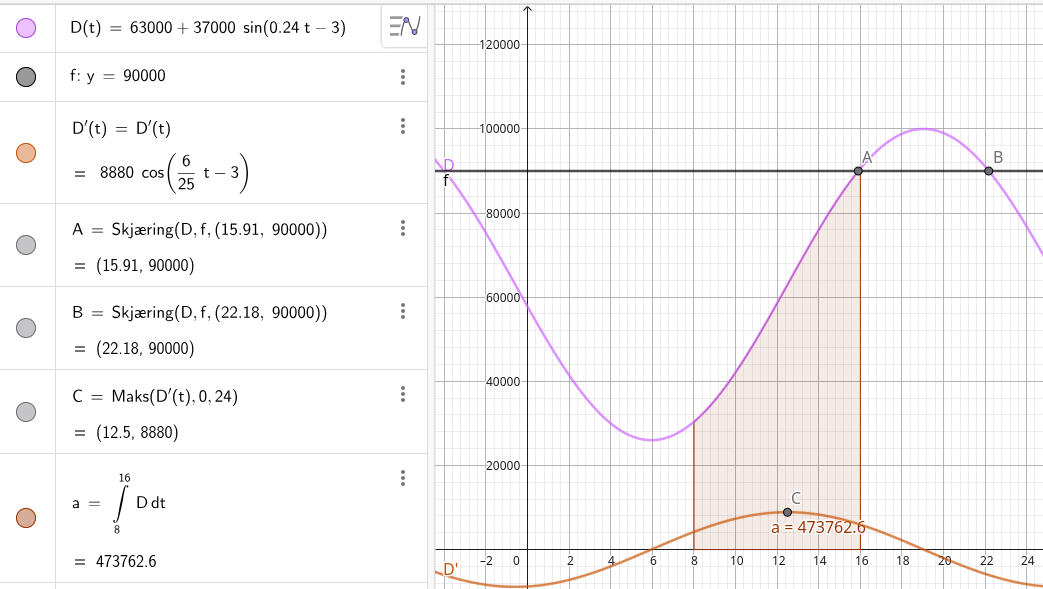
\includegraphics[scale=0.3]{opg1bcd	}
\end{figure}
\item Datatrafikken økte raskest når $D'(t)$ var størst. I rad 5 finner vi at dette var kl 12:30. Da var økningen 8\,880 gigabit per time per time.
\item Den totale datamengden mellom kl 8 og kl 16 er gitt ved integralet i rad 6. I løpet av arbeidsdagen ble det overført ca 473\,762 gigabit.
}

\subsection*{Oppgave 2}
\abc{
\item\phantom{'} \\ \pythonut{opg2.py}{
	5 \\
	16 \\
	225 \\
	50176 \\
	2517530625 \\
	6337960442777829376
}
\item Hvis $a_1>2$ eller $a_1<0$, er $a_n$ voksende, og da er ikke rekken konvergent. For $a_1=0$, $a_1=1$ og $a_1=2$ vil verdien til $a_n$ straks eller etterhvert svinge mellom 0 og 1, og da er ikke rekken konvergent. Følgelig er det ingen heltall for $a_1$ som gjør at rekken er konvergent.
}
\newpage
\subsection*{Oppgave 3}
\abc{
\item Vi definerer $\vec{r}(t)$ i CAS, og finner $z$-verdien til $\vec{r}$ etter 4 sekunder (celle 2). Da er flyet 18\enh{m} over motorveien.
\item Finner at når $z$-verdien til $\vec{r}$ er 0, er $t=18$ (celle 3). Banefarten er lengden til fartsvektoren. Når landet lander er banefarten ca. 10,31 \enh{m/s} (celle 4).
\item Banefarten er 14,3\enh{m/s} ca etter 8 sekunder og etter 20 sekunder (celle 5).
\item Vi definerer de to gitte punktene som $A$ og $B$ (celle 6 og 7), og finner $\vv{AB}$ (celle 8). Vi lar $\vec{p}(q)$ være posisjonen til fulgen $q$ sekunder etter at nødlandingen har starter. Ved å definere $\vec{p}(q)$ slik som i celle 9, er vi sikker på at grafen til $\vec{p}$ går gjennom $A$ og $B$, og at banefarten er $12\enh{m/s}$. For at flyet og fuglen skal treffe hverandre, krever vi at de har like koordinater til samme tid. I celle 10-12 finner vi at $x$- og $z$- koordinatene er tilnærmet like etter 5 sekunder. Differansene mellom $y$-verdiene når $t=q=5$ er ca. 0,22\enh{cm}. Med tanke på størrelsen til et fly og en fugl, er det da rimelig å anta at flyet og fuglen treffer hverandre etter 5 sekunder.
}
\begin{figure}
	\centering
	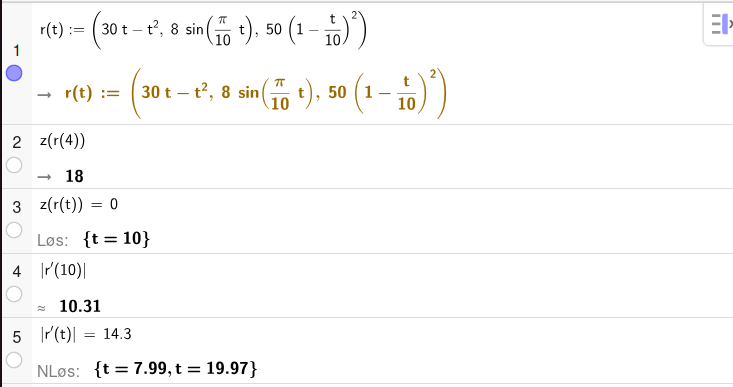
\includegraphics[scale=0.25]{opg3abc}\\
	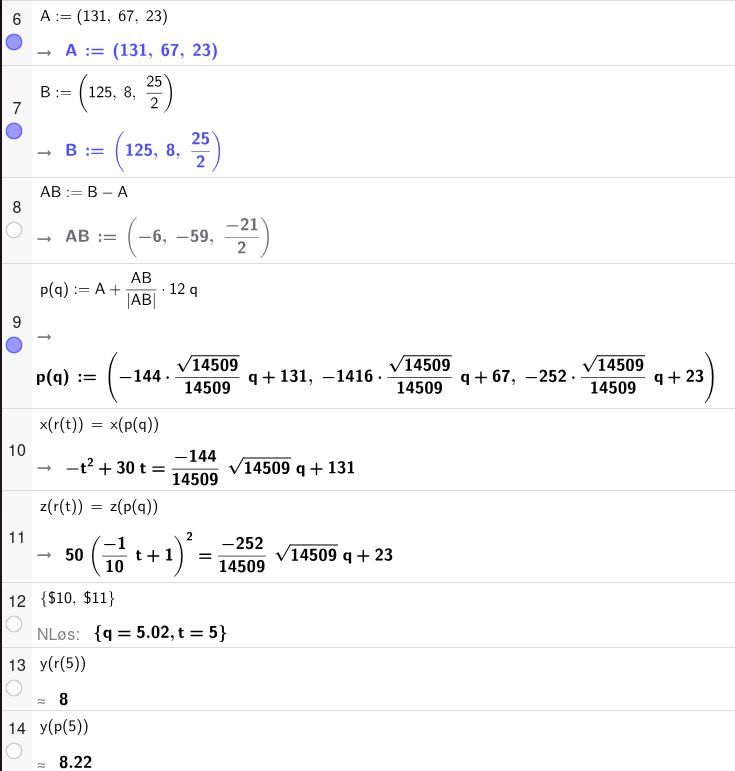
\includegraphics[scale=0.25]{opg3d}
\end{figure}
\newpage
\subsection*{Oppgave 5}
Vi tilnærmer vasens form ved en sinusfunksjon med vendepunkt i $x=0$ og $x=20$. Dette tilsvarer ''endepunktene'' til vasen, som dermed har høyde $20\enh{cm}$. Ved å sette amplituden til 0,5, og likevektslinja til $y=4,9$, får vi en vase med diameter $9,8\enh{cm}$ i topp og bunn, og som har $1\enh{cm}$ som differanse mellom sin tykkeste form og sin tynneste form. Av figuren og det resulterende integralet av omdreiningslegemet (rad 2) ser det ut som at $f$ er en grei tilnærming til vasen (rad 1).
\begin{figure}
	\centering
	
\includegraphics[scale=0.3]{opg5}
\end{figure}

\end{document} 